% Quantum Biology Atlas — Applications Note
%
% Built with a clean `article` class. The npj/Typst template used elsewhere in this
% portfolio is deliberately NOT reused: it hard-codes a fabricated DOI, volume and pages
% for in-preparation work into its .cls, whose \fancyfoot then stamps them onto every
% page of every document built from it.
%
% NO LITERAL NUMBERS APPEAR IN THIS FILE. Every quantity is a macro defined in
% numbers.tex, which scripts/build_manuscript_numbers.py generates from the build
% artefacts. If an analysis is re-run and a result moves, this manuscript moves with it.
\documentclass[11pt,a4paper]{article}

\usepackage[T1]{fontenc}
\usepackage[utf8]{inputenc}
\usepackage[margin=2.3cm]{geometry}
\usepackage{times}
\usepackage{graphicx}
\usepackage{booktabs}
\usepackage{caption}
\usepackage[sort&compress,numbers]{natbib}
\usepackage{xcolor}
\usepackage[hidelinks]{hyperref}
\usepackage{titlesec}

\captionsetup{font=small,labelfont=bf}
\titleformat{\section}{\normalfont\large\bfseries}{\thesection}{0.6em}{}
\titleformat{\subsection}{\normalfont\normalsize\bfseries}{\thesubsection}{0.6em}{}
\setlength{\parskip}{0.25em}
\bibliographystyle{unsrtnat}

% Generated by scripts/build_manuscript_numbers.py — do not edit.
%
% Every quantity the manuscript states is defined here from a build artefact.
% The body contains no literal numbers, so a re-run that moves a result moves
% the manuscript with it rather than leaving a stale figure in the text.

\newcommand{\NMaps}{10}
\newcommand{\NNodes}{126}
\newcommand{\NEdges}{168}
\newcommand{\NLoci}{125}
\newcommand{\NEntities}{83}
\newcommand{\NRefs}{42}
\newcommand{\NTierOne}{4}
\newcommand{\NTierTwo}{31}
\newcommand{\NTierThree}{44}
\newcommand{\NTierFour}{47}
\newcommand{\PctTierThreeFour}{72}
\newcommand{\QboVersion}{0.1.0}
\newcommand{\NSpecies}{5}
\newcommand{\OrthHuman}{68}
\newcommand{\OrthFly}{63}
\newcommand{\OrthHumanCorroborated}{22}
\newcommand{\PreregOR}{1.58}
\newcommand{\PreregP}{0.48}
\newcommand{\PreregMDE}{4.0}
\newcommand{\OsdTwentySevenContrasts}{5}
\newcommand{\OsdTwentySevenTesla}{16.5}
\newcommand{\OsdTwentySevenOrth}{63}
\newcommand{\OsdTwentySevenNodes}{15}
\newcommand{\OsdTwentySevenConsistent}{0}
\newcommand{\CryFly}{FBgn0025680}
\newcommand{\OsdEightTesla}{16.5}
\newcommand{\OsdEightLoci}{29327}
\newcommand{\OsdEightObs}{0.1660}
\newcommand{\OsdEightBg}{0.1763}
\newcommand{\OsdEightP}{0.705}
\newcommand{\OsdEightPerms}{10,000}
\newcommand{\OsdEightSymbolOnly}{17}
\newcommand{\RadDoses}{2}
\newcommand{\RadTimepoints}{4}
\newcommand{\RadLoci}{123}
\newcommand{\RadBestP}{0.87}
\newcommand{\RadMaxObs}{0.299}
\newcommand{\RadVsMagnetFold}{1.8}
\newcommand{\OverlapThreshold}{0.5}
\newcommand{\OverlapNnmfN}{11}
\newcommand{\OverlapNnmfShared}{4}
\newcommand{\OverlapNnmfAgree}{2}
\newcommand{\OverlapStrongN}{123}
\newcommand{\OverlapStrongObs}{3}
\newcommand{\OverlapStrongExp}{2.1}
\newcommand{\OverlapStrongP}{0.352}
\newcommand{\ParmLoci}{194}
\newcommand{\ParmCells}{2,716}
\newcommand{\ParmTimepoints}{7}
\newcommand{\AglLoci}{26}
\newcommand{\AglCells}{196}
\newcommand{\AglQbo}{7}


\newcommand{\repourl}{https://github.com/dr-richard-barker/quantum-biology-atlas}
\newcommand{\pagesurl}{https://dr-richard-barker.github.io/quantum-biology-atlas/}

\title{\vspace{-1.2cm}\textbf{Quantum Biology Atlas: evidence-tiered pathway maps for
magnetic-field effects in plants}}
\author{Richard Barker\thanks{Correspondence: \texttt{dr.richard.barker@gmail.com}}
\\ \small University of Wisconsin--Madison}
\date{}

\begin{document}
\maketitle
\vspace{-0.8cm}

% ---------------------------------------------------------------------------
\section*{Abstract}
\noindent\textbf{Summary:} Claims about magnetic-field effects in biology are easy to
draw and hard to qualify: a pathway diagram gives a hypothesised radical-pair site and a
measured one the same visual weight. The Quantum Biology Atlas separates the two
questions that are routinely conflated --- what quantum chemistry a molecular entity
carries, and how much is actually known about its field sensitivity --- and renders the
second as a border style, so a hypothesis looks provisional on the page. It publishes
\NMaps{} identifier-bound pathway maps (\NNodes{} annotated nodes, \NEdges{} edges,
\NLoci{} \emph{Arabidopsis} loci) as SBGN-ML \citep{LeNovere2009} with the quantum
annotation in extension blocks, a Python package that projects measured expression onto
them across \NSpecies{} species, and a browser tool that does the same for a user's own
table without uploading it. The overlay machinery refuses rather than degrades: a join
that matches nothing raises instead of rendering a pale map that looks like a result.
Applied to its own corpus the atlas returns two negatives that constrain how its figures
may be read, and reports both.

\smallskip
\noindent\textbf{Availability and implementation:} Source, ontology, maps and evidence
base at \url{\repourl}; interactive maps and the upload tool at \url{\pagesurl}. Code is
MIT; ontology, maps and evidence base are CC-BY-4.0.

\smallskip
\noindent\textbf{Contact:} \texttt{dr.richard.barker@gmail.com}

% ---------------------------------------------------------------------------
\section{Introduction}

The proposal that weak magnetic fields act on biology through spin-correlated radical
pairs is specific, testable and now well developed theoretically
\citep{Ritz2000,ZadehHaghighi2022}. In plants it has a named candidate receptor,
cryptochrome \citep{Ahmad2007,Solovyov2007,Pooam2019,Thoradit2023}, and a substantial
phenomenology: near-null fields alter flowering time, hypocotyl growth, reproductive
yield and mineral nutrition \citep{Xu2012,Xu2013,Agliassa2018a,Narayana2018,Islam2020}.

The gap is between those two bodies of work. The mechanism literature is about
chemistry; the phenomenology is about phenotypes; and pathway diagrams drawn to connect
them do not distinguish a site where a field effect has been \emph{measured} from one
where a plausible radical intermediate merely exists. Both appear as a box with an
arrow. That is not a presentation problem --- it is how a hypothesis acquires the
appearance of an established route.

The atlas addresses this narrowly. It does not adjudicate the mechanism. It makes the
evidence state of every node explicit, machine-readable and visible, and it makes
projecting real data onto those nodes the only way a number ever appears on a figure.

% ---------------------------------------------------------------------------
\section{Implementation}

\subsection{Two axes, kept orthogonal}

The ontology (QBO, version \QboVersion, \NEntities{} entities) annotates each entity on
two independent axes. \texttt{quantum\_class} records the chemistry it carries --- a
flavin semiquinone, a $[$2Fe-2S$]$ or $[$4Fe-4S$]$ cluster, a triplet ground state, a
site of reactive-oxygen leak. \texttt{evidence\_tier} records how much is known about its
magnetic-field sensitivity: T1 demonstrated, T2 inferred, T3 plausible, T4 context.

Collapsing these is the failure the design exists to prevent, and the validator enforces
their independence in both directions. A tier that asserts a demonstrated or inferred
field effect cannot validate without a DOI resolved against CrossRef --- the evidence
base holds \NRefs{} such references, each title-matched against the source ---; a T3 node cannot
validate without a written rationale. Conversely, an entity classed as structural
context \emph{may} carry a demonstrated effect --- iron uptake under near-null fields is
a measured phenomenon with no proposed mechanism \citep{Islam2020,Vigani2021} --- and the
validator requires only that the tension be stated, not that it be resolved.

\subsection{Tier as a visual channel}

Evidence tier is rendered as the node's border: heavy solid for T1, light solid for T2,
dashed for T3, hairline for T4. The consequence is that the atlas's own maps look mostly
provisional, because they are: of \NNodes{} nodes, \NTierOne{} are T1, \NTierTwo{} are
T2, \NTierThree{} are T3 and \NTierFour{} are T4 --- \PctTierThreeFour\,\% carry no
measured field effect at all. That is the finding rather than a defect. The near-null-field
literature is developmental and nutritional, and has not yet measured a respiratory
complex directly.

Maps are declarative sources carrying no coordinates; geometry is derived from measured
text metrics, so a label cannot outgrow its box. Rendering is checked by a probe that
runs in a real browser and asserts on what was painted --- no overlapping text, nothing
clipped, every overlay mark on its own node --- using the browser's own text layout
rather than re-running the compiler's arithmetic.

\subsection{Identifiers, which are where the joins actually fail}

Four of the six demonstrations needed a different identifier route, and each wrong
choice fails silently rather than loudly. Published supplementary tables write
\emph{Arabidopsis} loci as \texttt{At1g01980.1}, which a conventional AGI pattern
matches zero times. A two-colour array platform's \texttt{GENE\_SYMBOL} column holds a
locus only sometimes --- often a trivial name instead --- and reading it alone reaches
\OsdEightSymbolOnly{} of the atlas's \NLoci{} loci where the accession field reaches all
of them. Main-text tables are keyed on gene symbols, which cannot safely be resolved from
memory: authoring this ontology turned up five symbol collisions that would each have put
a different gene on a map, so symbols are resolved from each paper's own primer table.

\subsection{Projection, and what it refuses}

Measured values reach a figure only through \texttt{qbio.project}, from a named study and
a named contrast, with the provenance travelling into the caption. Three refusals are
enforced rather than warned:

\begin{itemize}\itemsep2pt
\item A join matching no node \textbf{raises}. A pale map rendered from nothing looks
  like a result, which is worse than an error.
\item Coverage below 25\,\% raises unless explicitly overridden, and the coverage is
  stated in the caption either way.
\item A series still on a ratio or signed-fold scale is refused. Published tables use at
  least three conventions, and feeding a ratio to a log$_2$ renderer colours every
  unchanged gene as strongly upregulated while looking entirely normal.
\end{itemize}

Cross-species projection runs two independent backbones --- Ensembl Compara
\texttt{pan\_homology} \citep{Cunningham2022} and a frozen OrthoDB matrix
\citep{Kuznetsov2022} --- and reports where they disagree rather than preferring one.
\OrthHuman{} of \NLoci{} loci reach human, of which \OrthHumanCorroborated{} are
called by both methods; \OrthFly{} reach \emph{Drosophila}, where only Ensembl can
reach --- the committed matrix is human-anchored, and the coverage report says so rather
than letting one method read as two. Unmapped
loci are listed, never dropped: the alternative oxidases fail to map to human because
humans do not have one, and that is a result.

\subsection{Time, and the limit of a node}

A time course is carried intact to the renderer and collapsed to one colour only at the
last moment, by largest-magnitude rather than mean: a gene that rises early and falls
late averages to ``no response''. Single-locus nodes carry a sparkline of the
trajectory. Multi-locus nodes do not --- they carry a per-locus heatmap instead, one row
per locus and one column per timepoint (Fig.~\ref{fig:main}D).

That choice was forced by a false positive. Under ionising radiation the alternative
oxidase node appeared to respond in the same direction as under a near-null field, a
clean shared result. At locus level AOX1D rises under both while AOX2 \emph{falls} under
radiation, and the aggregate was selecting a different family member at each timepoint.
Almost every multi-locus node behaves this way under a strong perturbation, so
\texttt{project\_series} now records per-timepoint sign divergence and the caption says
which nodes have it. A gene family is not a unit of response.

\subsection{Browser tool}\label{sec:browser}

\texttt{explore.html} performs the same join client-side, taking the shape of ShinyGO
\citep{Ge2020} but for hand-curated quantum-annotated maps rather than enrichment. The
file is read in the browser and never uploaded --- unpublished data should not have to
leave the machine to be looked at --- and the refusals above are ported intact and
rendered on the page, because a refusal that reaches only the console is not a refusal.

% ---------------------------------------------------------------------------
\section{Example}

\subsection{Demonstrations}

Six demonstrations span three provenance classes, which the atlas labels separately
because they do not carry equal weight: NASA GeneLab-processed differential expression
\citep{Berrios2021}, depositors' normalised ratios with no model fitted, and values read
from a paper's tables where nothing was deposited. The last class is necessary because
the group that produced most of the atlas's T1/T2 evidence deposited no raw data, and
each such page quotes the article's Data Availability Statement verbatim.

Several are worth naming. OSD-27 places a plant-anchored ontology on \emph{Drosophila} in a
\OsdTwentySevenTesla\,T magnet: \OsdTwentySevenOrth{} loci reach the fly, and
\emph{Arabidopsis} CRY1 lands on \texttt{\CryFly} --- the canonical animal
magnetoreceptor. Of $420$ contrasts, \OsdTwentySevenContrasts{} isolate field from the
effective gravity that diamagnetic levitation changes alongside it, and across those,
\OsdTwentySevenConsistent{} of \OsdTwentySevenNodes{} nodes move consistently. Parmagnani \emph{et al.}'s near-null time course \citep{Parmagnani2022} contributes
\ParmCells{} values across \ParmLoci{} loci at \ParmTimepoints{} timepoints in two
tissues, and Agliassa \emph{et al.}'s flowering series \citep{Agliassa2018a} adds
\AglCells{} values across \AglLoci{} loci, \AglQbo{} of them atlas nodes --- reaching
the hormone/circadian map that no repository dataset does. Mannino \emph{et al.}'s
near-null study in sweet basil (\emph{Ocimum basilicum}) \citep{Mannino2026}
contributes \ManninoCells{} values across \ManninoLoci{} loci, \ManninoQbo{} of them
atlas nodes on the redox map, demonstrating gene-metabolite decoupling in
phenylpropanoid metabolism alongside divergent regulation of superoxide dismutase
isoforms.

\subsection{Two negatives the atlas reports about itself}

\textbf{The selected loci are not preferentially field-responsive.} OSD-8 measures
\OsdEightLoci{} loci and contains the cleanest field-only contrast available:
\OsdEightTesla\,T inside a magnet against $0$\,T outside it at matched effective gravity.
The atlas's loci move by mean $|$log$_2$FC$|$ \OsdEightObs{} against \OsdEightBg{} for
the same number of loci drawn at random ($p=\OsdEightP$, \OsdEightPerms{} permutations).
All seven experimental groups agree, including two with no magnet in them.

This does not invalidate an ontology that selects for mechanism rather than observed
response, but it does constrain the figures: on this dataset, colour on a map is not
evidence that a field acts selectively at these nodes. The pre-registered test on the
corpus is likewise null (OR $\PreregOR$, $p=\PreregP$) with a minimum detectable odds
ratio of $\PreregMDE$ at 80\,\% power --- too underpowered to settle anything, which is
reported rather than omitted.

\textbf{The nodes are not inert, however.} A \RadDoses{}-dose,
\RadTimepoints{}-timepoint ionising-radiation series reaching \RadLoci{} of the atlas's
loci moves the same loci up
to \RadMaxObs{} mean $|$log$_2$FC$|$, roughly \RadVsMagnetFold$\times$ their response to
the \OsdEightTesla\,T field, while remaining below their background ($p \ge \RadBestP$).
So the magnetic null cannot be attributed to genes that do not move.

\subsection{Overlap between perturbations}

Radiation is not a magnetic-field regime and the atlas does not treat it as one; QBO's
field-regime vocabulary is not extended to it. But radiolysis makes radicals directly,
so the question of overlap is worth asking. Of \OverlapNnmfN{} loci measured under both
ionising radiation and a near-null field --- a locus counting as responding at
$|$log$_2$FC$| \ge \OverlapThreshold$, applied identically to both sides so the overlap
cannot be tuned --- \OverlapNnmfShared{} respond to both and
\OverlapNnmfAgree{} agree in direction. That is reported as a table and explicitly not
tested: below twenty shared units the permutation test refuses rather than returning a
$p$-value that would read as evidence. Against the strong-field study, where
\OverlapStrongN{} loci are shared and a test is possible, the observed overlap of
\OverlapStrongObs{} against \OverlapStrongExp{} expected is unremarkable
($p=\OverlapStrongP$).

\begin{figure}[p]
\centering
\begin{minipage}{0.56\textwidth}\centering
  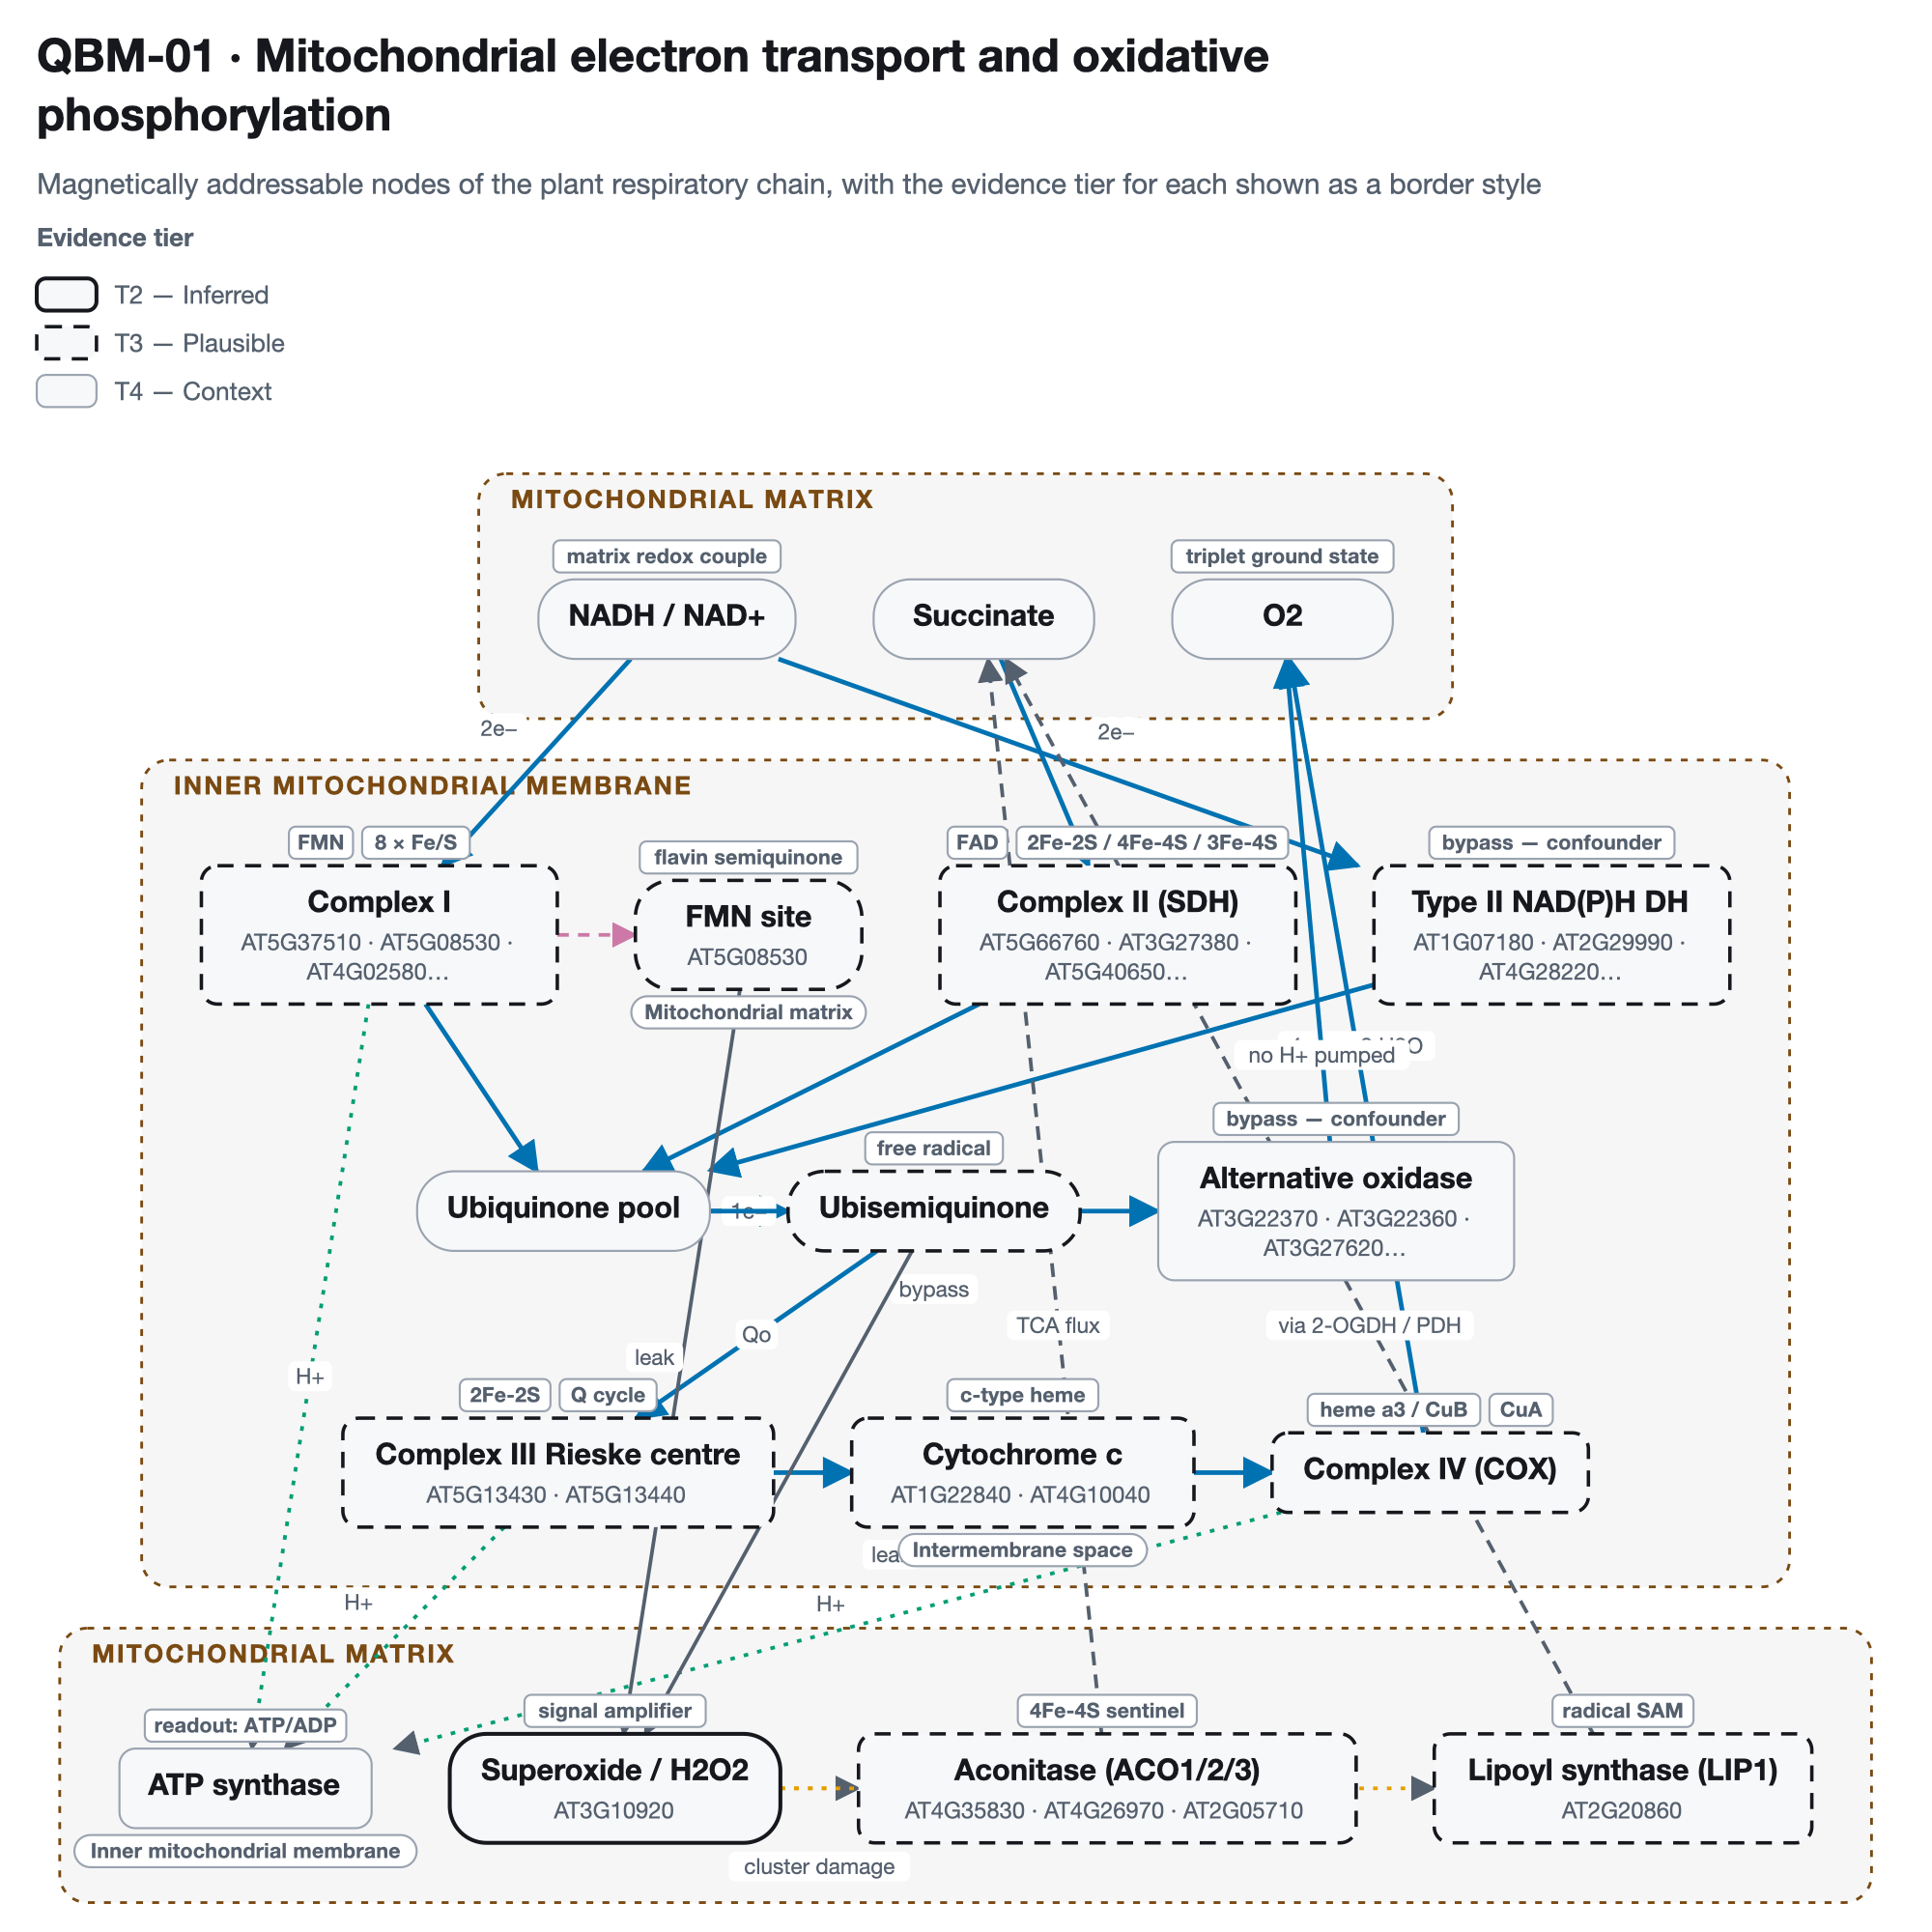
\includegraphics[width=\linewidth,trim=0 0 0 0,clip]{figures/panelA.png}\\[2pt]
  {\small\textbf{(A)}}
\end{minipage}\hfill
\begin{minipage}{0.41\textwidth}\centering
  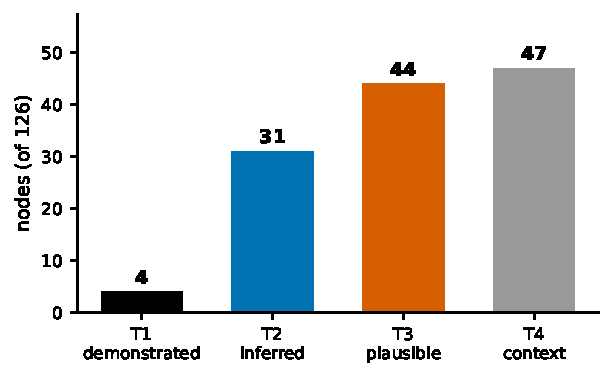
\includegraphics[width=\linewidth]{figures/panelB.pdf}\\[2pt]
  {\small\textbf{(B)}}
\end{minipage}

\vspace{0.5em}
\begin{minipage}{0.48\textwidth}\centering
  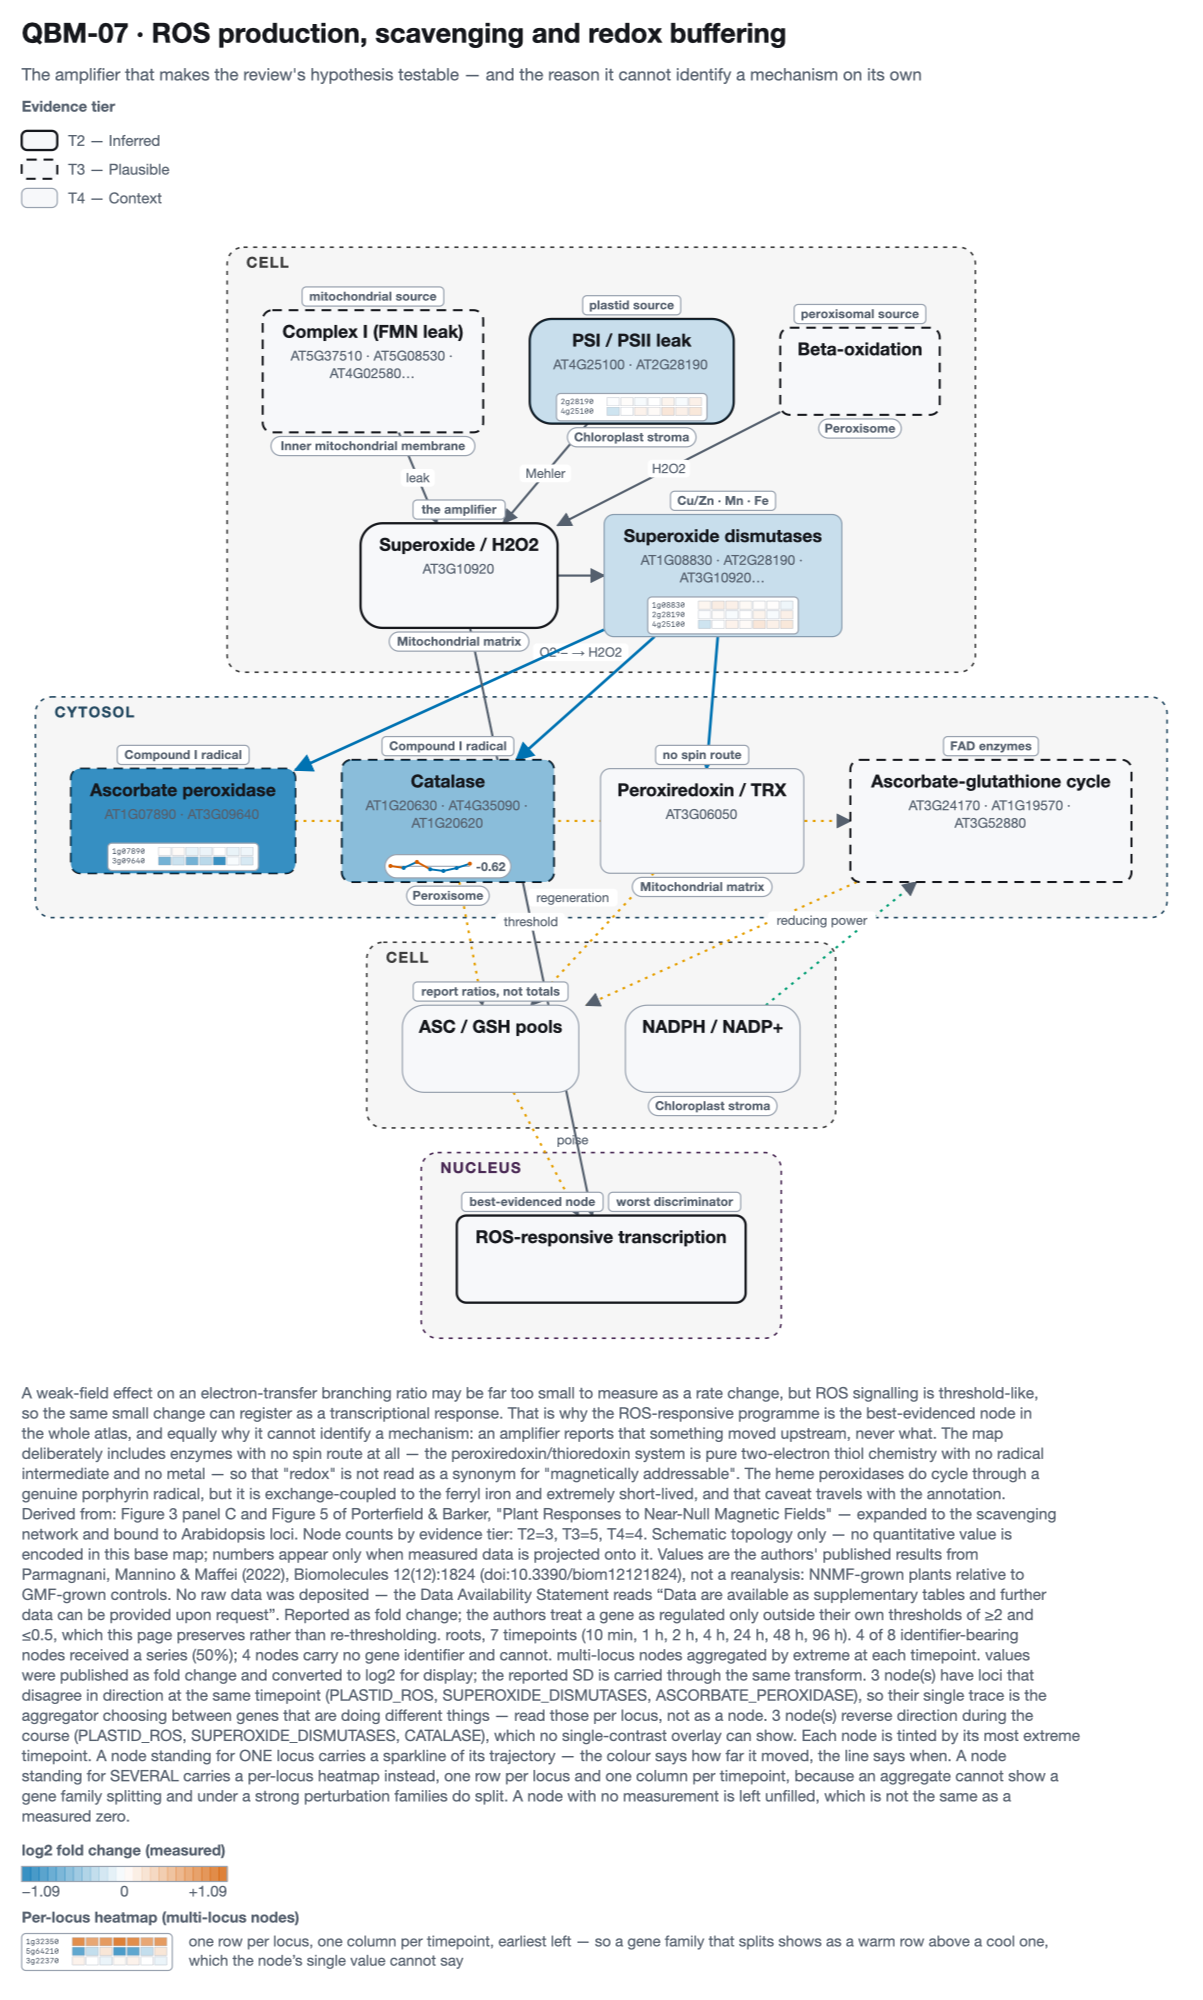
\includegraphics[width=\linewidth]{figures/panelC.png}\\[2pt]
  {\small\textbf{(C)}}
\end{minipage}\hfill
\begin{minipage}{0.48\textwidth}\centering
  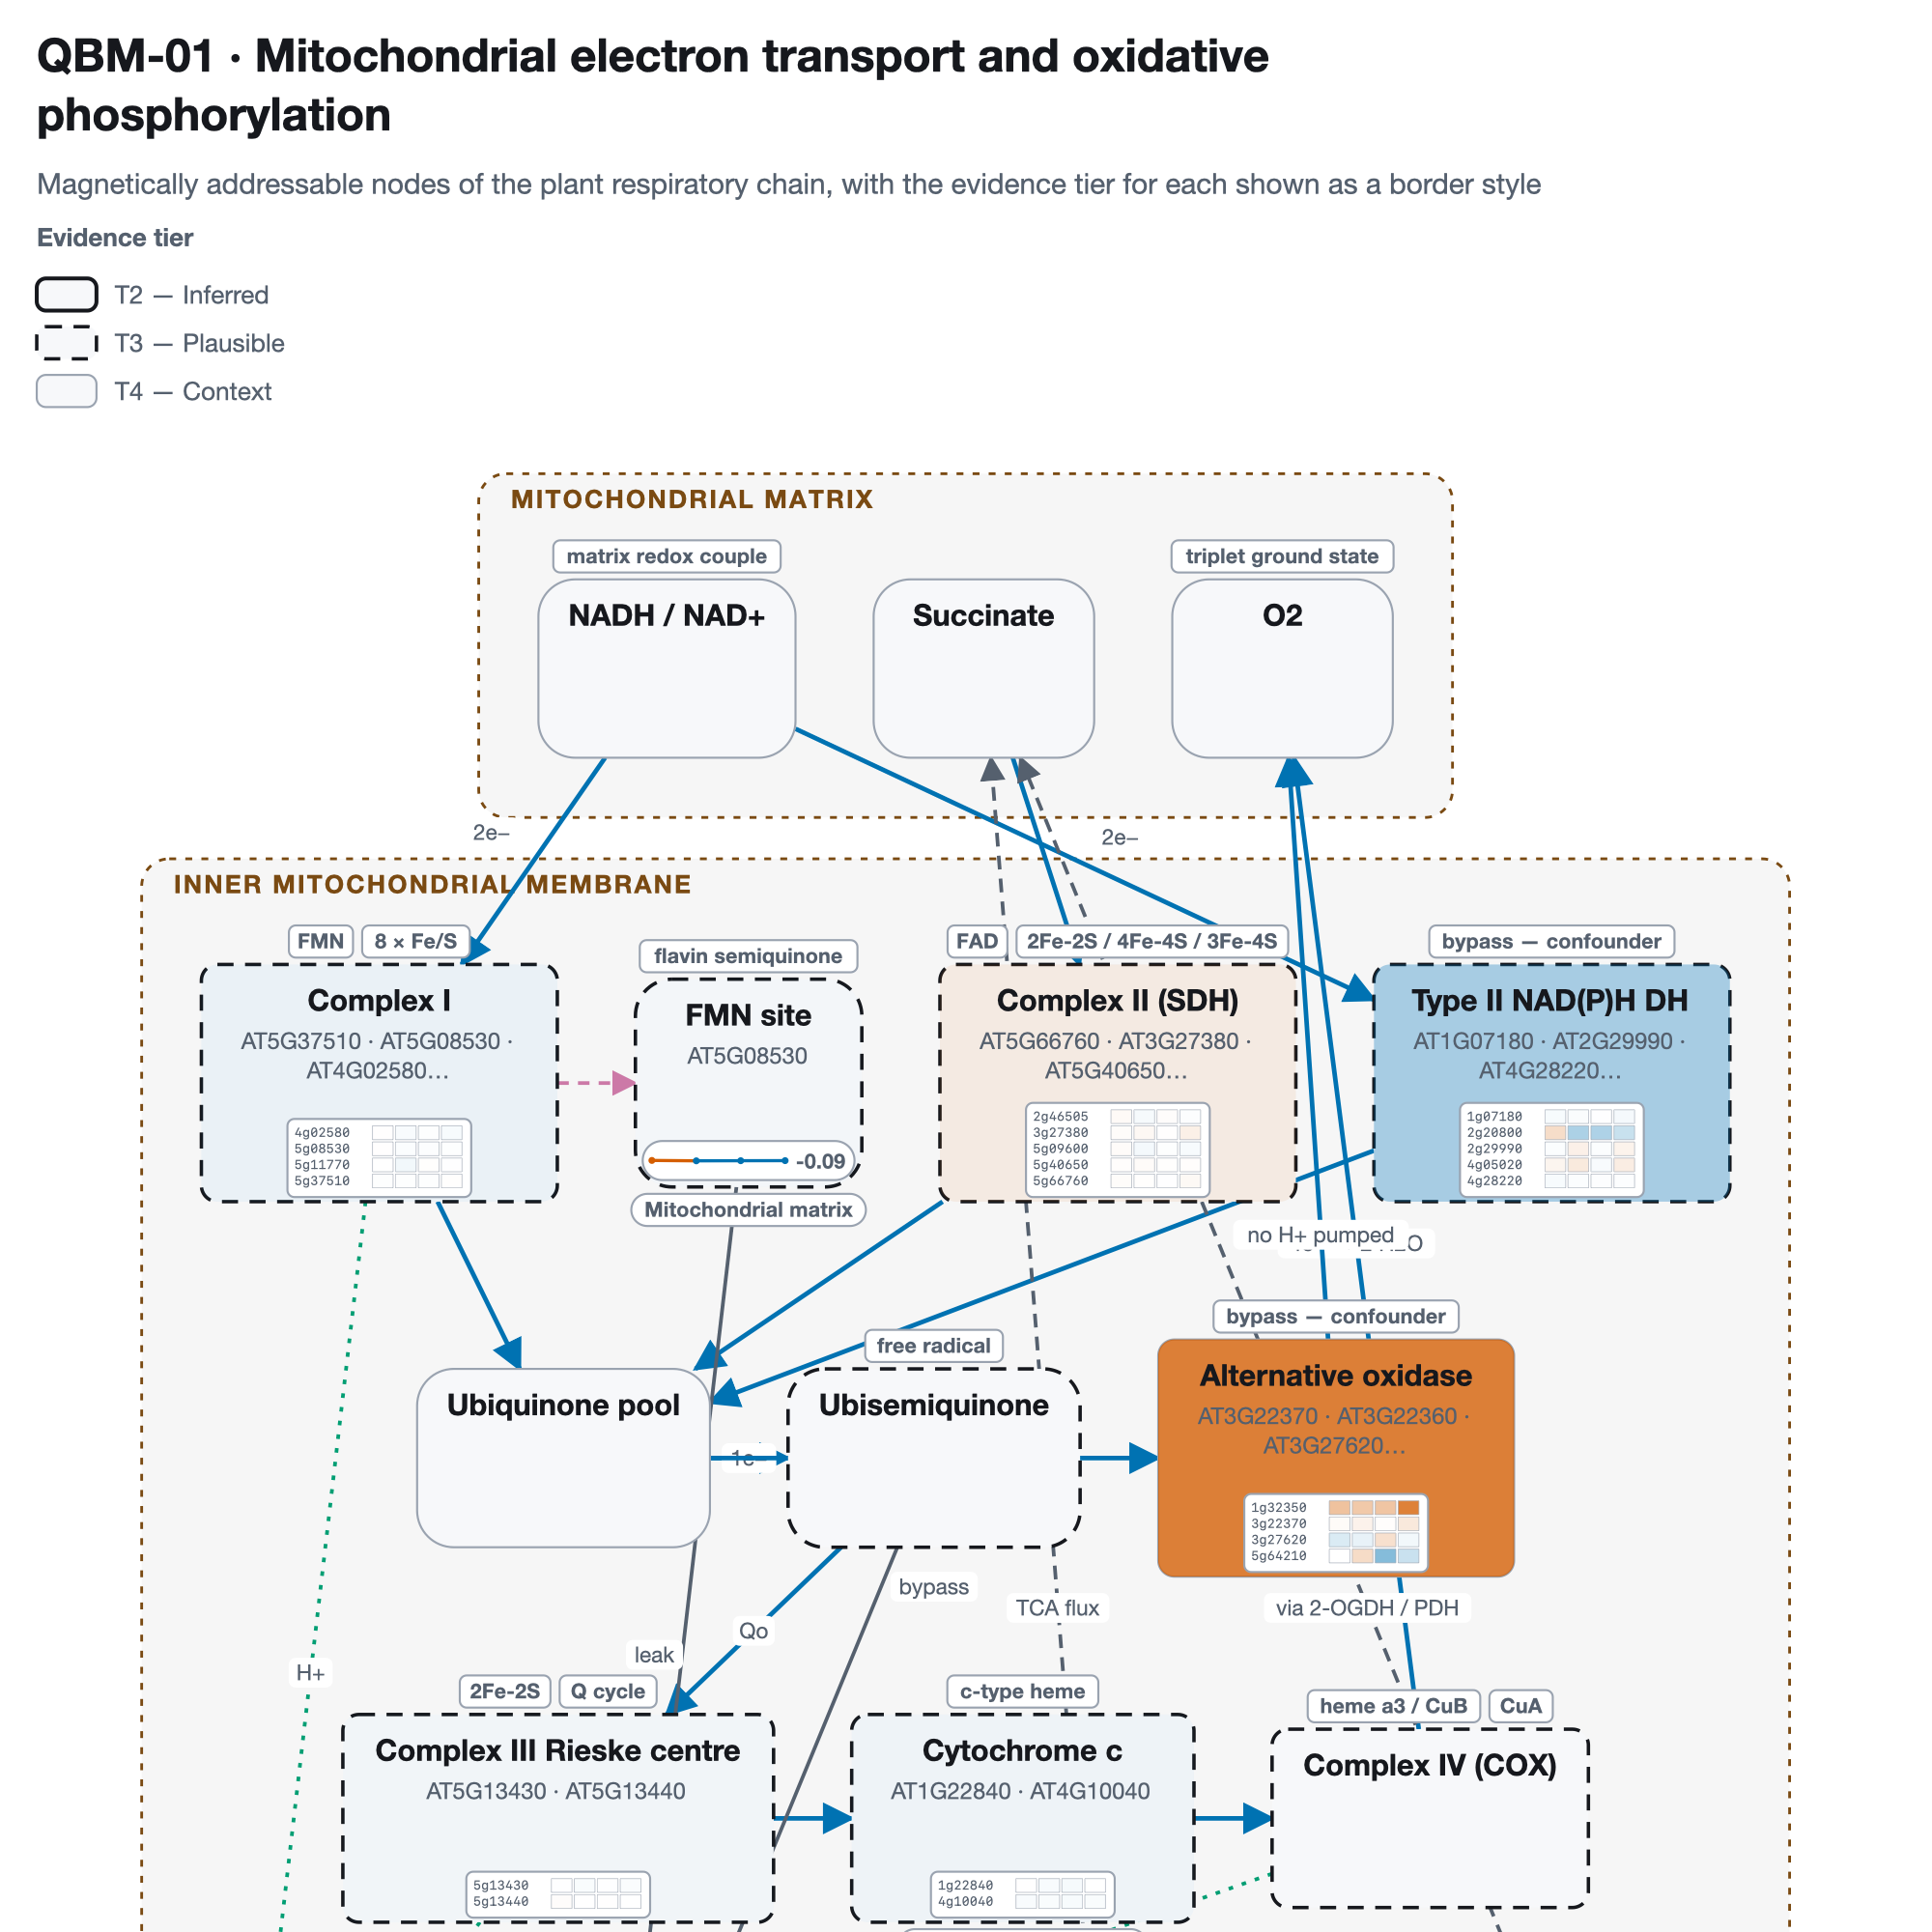
\includegraphics[width=\linewidth]{figures/panelD.png}\\[2pt]
  {\small\textbf{(D)}}
\end{minipage}

\caption{\textbf{The atlas and its outputs.}
\textbf{(A)} QBM-01, the mitochondrial electron transport map, with evidence tier as a
border channel: heavy solid T1, light solid T2, dashed T3, hairline T4. Most of the map
is dashed.
\textbf{(B)} Distribution of the \NNodes{} nodes across tiers --- \PctTierThreeFour\,\%
are T3 or T4, which is the state of the literature rather than a limitation of the
corpus.
\textbf{(C)} A near-null-field time course \citep{Parmagnani2022} projected onto the
redox map; single-locus nodes carry a sparkline of the trajectory.
\textbf{(D)} The same machinery under ionising radiation, where multi-locus nodes carry
a per-locus heatmap instead --- one row per locus, one column per timepoint. This is
what reveals a gene family splitting, which the aggregate hides.
Every panel is a file the repository generated; none was drawn. The browser tool is
described in Section~\ref{sec:browser} rather than shown, because illustrating it would mean a
screenshot rather than an artefact.}
\label{fig:main}
\end{figure}

% ---------------------------------------------------------------------------
\section{Conclusion}

The atlas is infrastructure for a field whose central claim is not settled, and its value
is in making the unsettledness legible: which nodes carry which chemistry, what is
actually known about each, and what a given dataset does and does not show. Its own two
negatives are part of the output rather than an embarrassment --- a tool that only
reported confirmations would be the wrong tool for this literature.

Distribution is by PyPI, GitHub Pages and Zenodo rather than Bioconductor. The atlas is
Python and TypeScript where Bioconductor is an R ecosystem; the rendering niche is
already occupied by \texttt{SBGNview} and \texttt{pathview}; and ShinyGO, the tool this
one is shaped after, is not a Bioconductor package either. A thin R annotation-data
package exposing the QBO corpus to those renderers would be the novel layer without the
competing one, and remains open.

\subsection*{Acknowledgements}
The companion review \citep{PorterfieldBarker} is in preparation and has no DOI; none is
recorded here.

\bibliography{references}
\end{document}
